\chapter{DATU ANALĪZE UN IEGŪTIE REZULTĀTI}




%\section{Novērojuma viekšana?}

\section{Novērojuma apstrāde} \label{data-process}
Novērojuma apstrādes procesu var sadalīt vairākos soļos, katrā solī iegūstot rezultātu. Nodaļā, kā piemērs, tiks apskatīts komētas ATLAS Y4/2019 novērojumu datu rezultāti no 15. marta novērojumu sesijas.
Komētas novērojumi tika plānoti, balstoties uz \ref{planning} nodaļā aprakstītajiem plānošanas soļiem, bet iegūtie novērojuma dati tika apstrādāti balstoties uz 1. nodaļā aprakstītās metodikas. 

\begin{wraptable}{l}{0.5\textwidth}
        \caption{Nodaļā aprakstītā novērojuma informācija}
    \centering
        \begin{tabular}{|l|l|}
        \hline
        Identifikators & atlas\_r\_f1666\_ir\_1 \\ \hline
        Sākuma laiks   & 2020-03-15T04:18:08    \\ \hline
        Beigu laiks    & 2020-03-15T06:34:16    \\ \hline
        Skanu daudzums & 120                    \\ \hline
        FFT garums     & 4096                   \\ \hline
        Joslas platums & 32 MHz                 \\ \hline
        Kanāla platums & 1.526 KHz              \\ \hline
        \end{tabular}
        \label{tab:example-atlas}
\end{wraptable}

Konkrētais novērojums ir izvēlēts kā piemērs, jo ir iespējams attēlot visus 1. nodaļā aprakstītos datu apstrādes soļus. Novērojumam ir pieejami gan jēldati, gan dat formāta faili, kā arī dažos skanos ir detektējamas anomālijas. Novērojuma aktuālā informācija aprakstīta tabulā \ref{tab:example-atlas}.





%\begin{table}[h!]
%\centering
%\begin{tabular}{|l|l|}
%\hline
%Identifikators & atlas\_r\_f1666\_ir\_1 \\ \hline
%Sākuma laiks   & 2020-03-15T04:18:08    \\ \hline
%Beigu laiks    & 2020-03-15T06:34:16    \\ \hline
%Skanu daudzums & 120                    \\ \hline
%FFT garums     & 4096                   \\ \hline
%Joslas platums & 32 MHz                 \\ \hline
%Kanāla platums & 1.526 KHz              \\ \hline
%\end{tabular}
%\caption{Nodaļā aprakstītā novērojuma informācija}
%\label{tab:example-atlas}
%\end{table}

Pirmais iegūtais grafiku tips datu apstrādes procesā ir amplitūdu grafiks, kas ir ticis iegūts, balstoties uz \ref{read-data} nodaļā aprakstītās datu nolasīšanas algoritma. Nolasot visus datus, rezultāti tiek attēloti informatīviem mērķiem un minētās novērojumu sesijas gadījumā tiek iegūti divi grafiki, katrs savam datu tipam (skatīt attiecīgi attēlos \ref{fig:raw-data-atlas}, \ref{fig:dat-data-atlas}). Papildus, rezultātus var izmantot, lai identificētu anomālijas jau pirmajā novērojumu apstrādes fāzē. 

\begin{figure}[H]
\centering
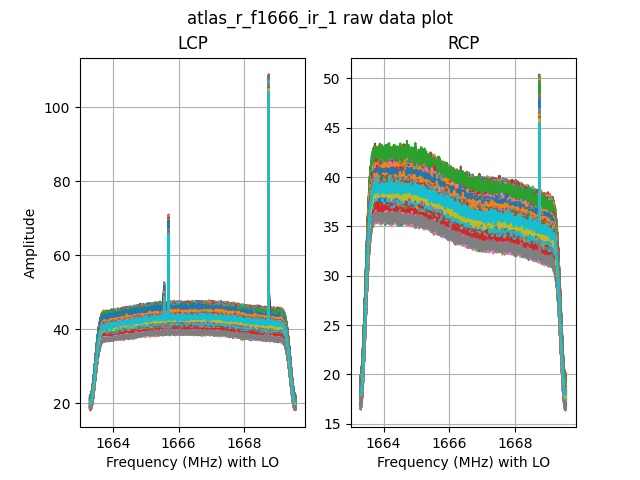
\includegraphics[width=\textwidth]{images/created/atlas-r-f1666-ir-1-raw.png}
\caption{Jēldatu nolasīšanā iegūtais rezultāts}
\label{fig:raw-data-atlas}
\end{figure}

Grafikos \ref{fig:raw-data-atlas}, \ref{fig:dat-data-atlas} attēlotas abas cirkulārās polarizācijas, kā arī visu skanu rezultāti pēc datu nolasīšanas. Rezultātu attēlošanā uz y ass tiek norādīta amplitūda, bet uz x ass - frekvence. Rezultātu iegūšanas brīdī, aprēķini tiek veikti neizmantojot lokālo oscilatoru, taču šiem rezultātiem lokālā oscilatora vērtība tiek pieskaitīta, lai ērtāk orientētos frekvenču joslā. Lai gan novērojumu sesijā vienlaicīgi tiek iegūti abi datu formāti, teleskopu tehnisku grūtību dēļ, iegūtie rezultāti labajā cirkulārajā polarizācijā ir atšķirīgi. Individuālie grafiki apzīmē iegūto rezultātu katrā skanā, līdz ar to katrā polarizācijā ir iegūti 120 spektri.



\begin{figure}[H]
\centering
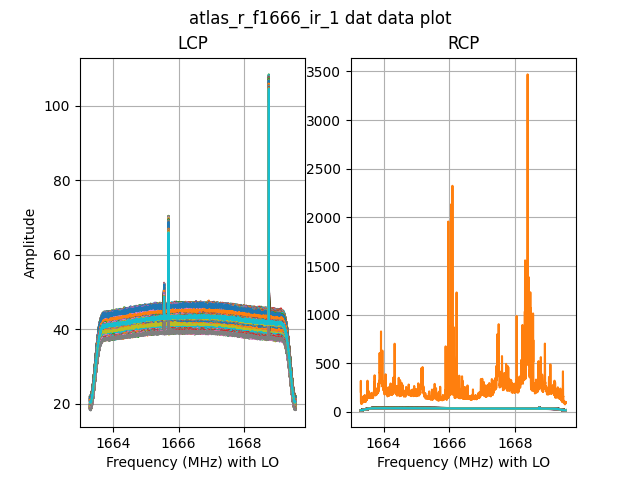
\includegraphics[width=\textwidth]{images/created/atlas-r-f1666-ir-1-dat.png}
\caption{Dat formāta datu nolasīšanā iegūtais rezultāts}
\label{fig:dat-data-atlas}
\end{figure}


Apstrādājot dat failus, iegūtas amplitūdas vērtības norāda, ka novērojuma laikā ir bijušas tehniskas problēmas, jo kreisajā cirkulārajā polarizācijā tiek iegūtas daudz augstākas vērtības noteiktos skanos, salīdzinot ar citiem skaniem. Minētās amplitūdas svārstības netika novērotas jēldatu apstrādes rezultātā, kur iegūtais spektrs nav bojāts, taču tas nenozīmē, ka šiem datiem nav nekādu problēmu. Izmantojot Furjē transformāciju, var iegūt amplitūdu pīķus frekvencēs, kurās avots staro. Pēc spektrālo līniju apraksta \cite{spectral-lines}, OH spektrālajām līnijām ir konkrētas frekvences, kurās OH māzeri staro, līdz ar to, ideālā gadījumā, pīķi būtu novietoti 1665.402 MHz un 1667.359 MHz vērtībās. Aprakstītajā novērojumu sesijas gadījumā ir novērots arī kāds parazītisks signāls, kurš staro citās, bet tuvās frekvenču vērtībās, spēcīgāk par meklēto OH māzeri, kurās pīķis parādās un ietekmē rezultātus.


Lai tālāk analizētu iegūtos datus, ir nepieciešams apskatīt novērojuma sistēmas temperatūras vērtībās. Balstoties uz formulām \ref{eq:1.2.2} un \ref{eq:1.2.3}, kuras aprakstītas \ref{calibration} nodaļā, tiek iegūts \ref{fig:tsys-atlas-raw} attēla grafiks. Bakalaura darba nodaļas ietvaros ir attēlots tikai jēldatu iegūtais rezultāts, jo dat failu rezultāts ir ļoti līdzīgs. Grafikā attēlotas sistēmas temperatūra Kelvinos katrā skana izpildē, kur \textit{LCP ref} un \textit{LCP sig} - kreisās cirkulārās polarizācijas references un objekta sistēmas temperatūras spektri, bet \textit{RCP ref} un \textit{RCP sig} - labās cirkulārās polarizācijas references un objekta sistēmas temperatūras spektri.



%tsys plot
\begin{figure}[H]
\centering
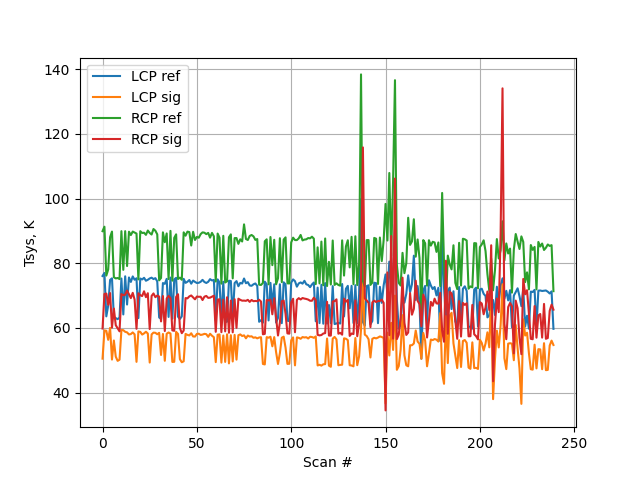
\includegraphics[width=\textwidth]{images/created/tsys-raw-atlas-1.png}
\caption{Jēldatu formāta novērojumā aprēķinātā sistēmas temperatūra}
\label{fig:tsys-atlas-raw}
\end{figure}

Attēlojot sistēmas temperatūras vērtības grafiski, viegli ieraudzīt pēkšņas sistēmas temperatūras izmaiņas. Skani, kuros sistēmas temperatūra pārsniedz normu, spēcīgi negatīvi ietekmēs rezultējošo plūsmas blīvuma spektru, kurš tiek iegūts nākamajā datu apstrādes solī. Pēc \ref{anomalies} nodaļā aprakstītās metodikas, iespējams detektēt minētās izmaiņas algoritmiski. Sākotnēji bojātie skani netika ņemti vērā jēldatu apstrādē, tāpēc bija iespējams apstrādāt mazāku daudzumu datus. Līdz ar to, pareģojot bojāto sistēmas temperatūras vērtību, ir iespējams joprojām izmantot ierakstītos datus.

Izmantojot veivletu transformāciju, var iegūt spektra formu, kura vērtības iespējams izmantot bojātu sistēmas temperatūru gadījumos. Nodaļā aprakstītais rezultāts iegūts izmantojot \textit{rbio1.5} veivletu ar slieksni 3, kas arī ir noklusējuma konfigurācijā. Nodaļā aprakstītā piemēra gadījumā bojātie dati ir detektēti skanos 137, 138, 150, 152, 153, 154, 155, 169, 179, 180, 181, 206, 207, 211, 212, 222. Neizmantojot aprakstīto metodi, bet saglabājot datu integritāti, būtu nepieciešams neapstrādāt 12 skanus jeb 10\% no visiem novērojuma skaniem. Pēc anomāliju detektēšanas un vērtību aizvietošanas, tiek iegūts grafiks \ref{fig:tsys-atlas-modified}, kur papildus grafika \ref{fig:tsys-atlas-raw} sistēmas temperatūras spektriem attēlots arī veivletu transformācijā iegūtie spektri katram sistēmas temperatūras grafikam. Visas iepriekš detektētās skanu sistēmas temperatūras vērtības ir aizvietotas ar vievletu transformācijas rezultējošo vērtību.


\begin{figure}[H]

\centering
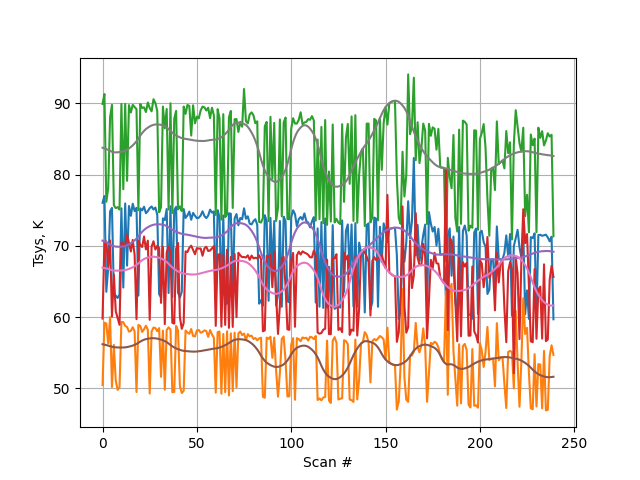
\includegraphics[width=\textwidth]{images/created/atlas-r-f1666-ir-1-tsys-edited.png}
\caption{Jēldatu aprēķinātā sistēmas temperatūra pēc anomāliju identificēšanas}
\label{fig:tsys-atlas-modified}
\end{figure}

Kad iegūtas derīgas sistēmas temperatūras vērtības, ir iespējams kalibrēt \ref{fig:raw-data-atlas} un \ref{fig:dat-data-atlas} grafikos iegūtos rezultātus pēc \ref{calibration} nodaļā aprakstītās metodikas. Kalibrācijas procesā iegūtais rezultāts attēlots \ref{fig:atlas-1-flux} grafikā, kur attēlots abu polarizāciju spektrālās plūsmas blīvums atkarībā no frekvences, izmantojot novērojuma jēldatus. Iegūtais rezultāts no dat tipa datiem ir ļoti līdzīgs, līdz ar to atskaitē nav apskatīts. Salīdzinot attēlos \ref{fig:raw-data-atlas} un \ref{fig:dat-data-atlas} iegūto frekvenču joslu, rezultējošā frekvenču josla ir mazāka, jo interesējošais spektrs ir izgriezts no kopējā. Ar raustītām sarkanām līnijām ir iezīmētas OH māzeru spektrālās līnijas. Ideālā scenārijā, iezīmētājās frekvencēs iespējams iegūt pīķi, 3 reizes izteiktāku par pārējo troksni, bet viena novērojuma rezultātos diemžēl nav iespējams iegūt tik precīzas vērtības apskatītajam objektam.

\begin{figure}[H]
\centering
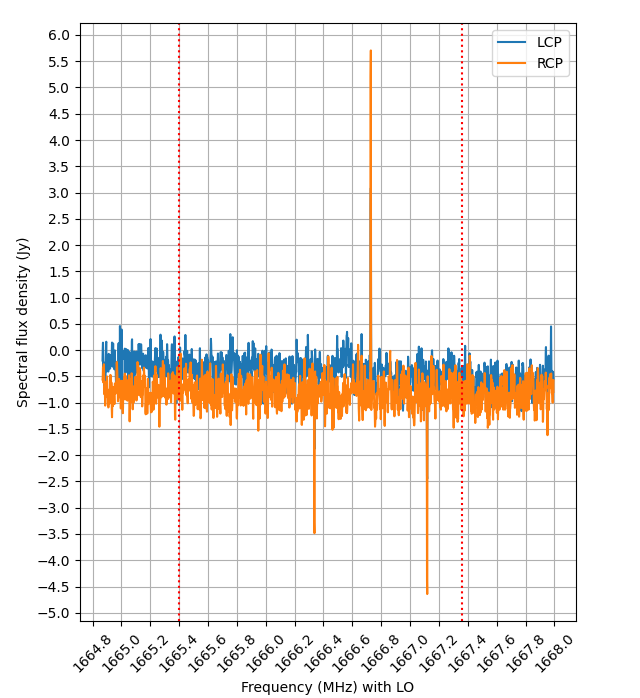
\includegraphics[width=\textwidth]{images/created/atlas-r-1-flux.png}
\caption{Spektrālās plūsmas blīvums atlas-r-f1666-ir-1 datiem.}
\label{fig:atlas-1-flux}
\end{figure}



Izmantojot iepriekš zināmo informāciju, iespējams aprēķināt trokšņa līmeni novērojumā pēc formulas


\begin{equation}
dS = \frac{SFED}{\sqrt{RBW \cdot t}} \tag{2.3.1}\label{eq:2.3.1} 
\end{equation}
kur: 
\begin{tabbing}
\phantom{\hspace{15mm}}\= \kill
$SEFD$\> = Teleskopa jūtība \\
$t$\>   = Novērojuma integrācijas laiks \\
$dS$\>   = Mērījuma troksnis \\
$RBW$\> = Kanāla platums\\

\end{tabbing}

Pēc iekšējā pētījuma rezultātiem \cite{telescope-sefd}, pieņemot, ka teleskopa jūtība ir 700 Jy, kā arī pieņemot, pēc 3 sigmu likuma, ka, lai objektu detektētu, minimālajam objekta plūsmas jaudai jābūt vismaz 3 reizes spēcīgākam par mērījuma troksni, šajā novērojumu iterācijā iegūst aprēķinu:



\begin{equation}
Sf = 3 \cdot dS = 3 \cdot \frac{700 (Jy)}{ \sqrt{1526 (Hz) \cdot 7200 (s) } }\approx 3 \cdot 0.211 (Jy) \approx 0.634 (Jy) \tag{2.3.2}\label{eq:2.3.2} 
\end{equation}
kur: 
\begin{tabbing}
\phantom{\hspace{15mm}}\= \kill
$Sf$\> = Avota spilgtums \\
$dS$\>   = Mērījuma troksnis pēc formulas \ref{eq:2.3.1}\\

\end{tabbing}




\section{Iegūto rezultātu izvērtējums} \label{result-eval}
%Salīdzināšana ar citu zinātnisko avotu rezultātiem, pārbaudes utt.




 %Aprakstīt rezultātus no ATLAS
Balstoties uz to, ka viena novērojuma rezultātā, ar patreizējām tehnoloģijām nevar detektēt signālu, pēc \ref{doppler} nodaļā aprakstītās metodikas iespējams apvienot vairākus novērojumu rezultātus. 

Apskatot iepriekšējā nodaļā novēroto objektu ATLAS Y4/2019 ilgākā laika periodā pēc teorijas iespējams mazināt kopējo trokšņa līmeni novērojumā. Ņemot vērā, ka objekta sadalīšanās veido rezultātu nestabilitāti, ar pielieto metodiku nav iespējams detektēt signālu. Lai iegūtu vairāk informācijas par objektu, ir nepieciešams apskatīt iegūtos datus noteiktos intervālos, kas Bakalaura darba ietvaros nav apskatīts. Lai iegūtu loģisko turpinājumu iepriekšējā nodaļā aprakstītajiem rezultātiem, tiek apskatīts 133 stundu laikā iegūto datu apkopojums jeb 37 dažādu novērojumu rezultāts, atspoguļots \ref{fig:atlas-individ} attēlā, kur ar gradienta palīdzību vecākie dati attēloti, izmantojot gaiši zilu krāsu, bet jaunākie - apzīmēti ar tumši zilu. Pats jaunākais novērojums atzīmēts atsevišķi ar violetu krāsu.
Bakalaura darba atskaitē tiek apskatīta tikai kreisās polarizācijas, 1667 MHz daļas dati, taču iegūtais rezultāts ir pielīdzināms arī pārējām novēroto datu daļām.
\begin{figure}[H]
\centering
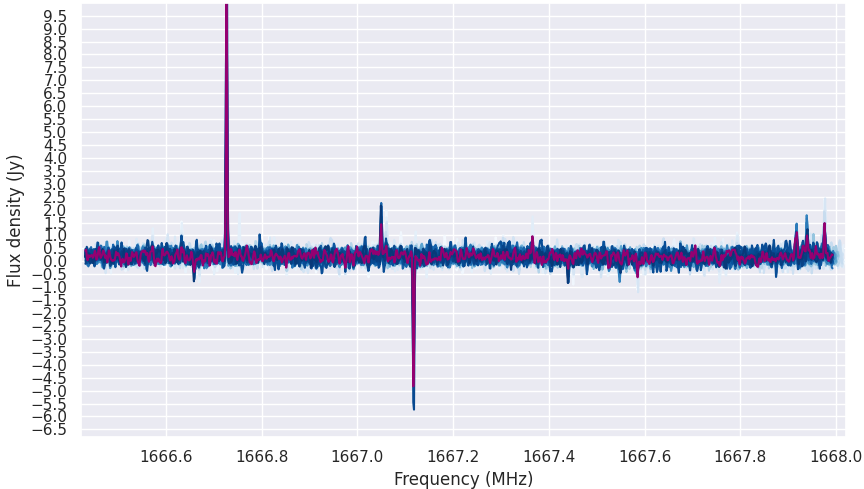
\includegraphics[width=\textwidth]{images/created/atlas-individ.png}
\caption{Visu individuālo novērojumu rezultāts ATLAS Y4/2019 komētas kreisajai cirkulārai polarizācijai.}
\label{fig:atlas-individ}
\end{figure}


Izmantojot attēlā \ref{fig:atlas-individ} iegūtos rezultātus, nav iespējams detektēt signālu nevienā no individuālajiem novērojumiem, līdz ar to, apvienojot visus novērojumus, iegūst \ref{fig:atlas-combined} attēlu, kur reprezentēts interesējošais apgabals kreisās cirkulārās polarizācijas 1667 MHz datu apgabalā, kā arī ar sarkanu līniju iezīmēta OH māzeru starošanas frekvence. Lai gan zemās pīķa maksimālā vērtības dēļ, datu apstrādes rezultāts nevar tikt uzskatīts kā neapstrīdams, ir iespējams, ka tiek detektēts signāls, taču Bakalaura darba ietvaros padziļināti apstrādes rezultāti netiek apskatīti. 

\begin{figure}[H]

\centering
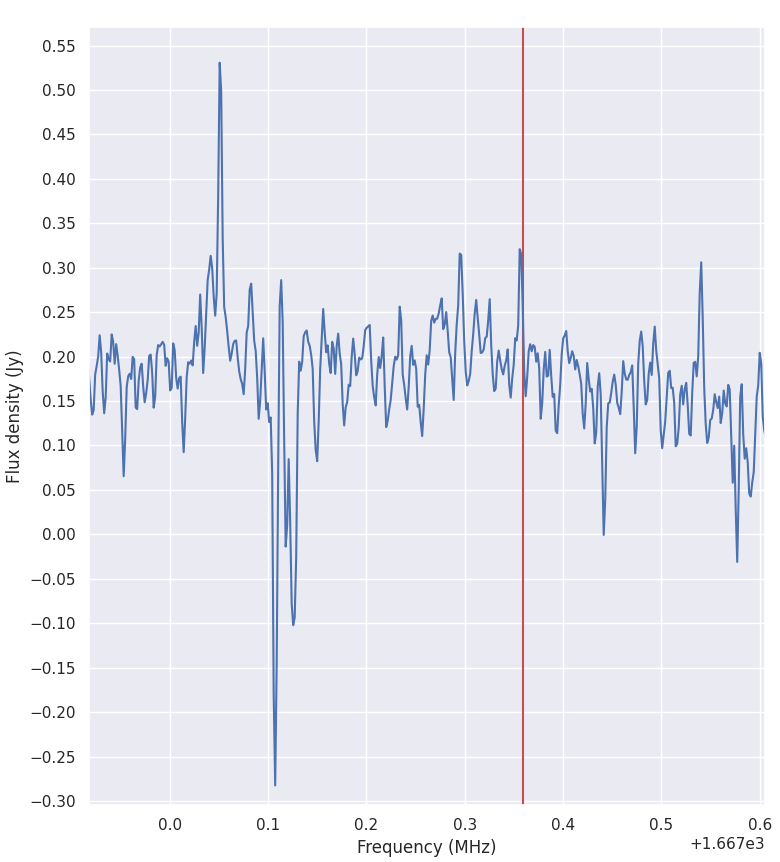
\includegraphics[width=\textwidth]{images/created/1667-atlas-found.png}
\caption{Plūsmas blīvuma atkarība no objekta frekvences ATLAS Y4/2019 kreisās cirkulārās polarizācijas datiem.}
\label{fig:atlas-combined}
\end{figure}




Lai gan komētu novērošanā vēl ir daudz darba, Bakalaura darba ietvaros ir veikts liels progress citu vāju objektu novērošanā. Atsaucoties uz \ref{wavelets} nodaļā aprakstītajiem RLMi rezultātiem attēlā \ref{fig:rlmi-boxed}, izmantojot izveidoto metodiku ir iegūti daudz pārliecinošāki rezultāti. Rezultātus tieši nedrīkst salīdzināt, jo ir daudz ietekmējoši faktori, it īpaši novērojuma ilgums un joslas platuma izmaiņas, taču iegūtie rezultāti liecina, ka objektu var detektēt novērojumu datos ar augstu ticības līmeni.

RLMi maiņzvaigznes patreizējā novērošanas iespējamība attēlota \ref{fig:rlmi-doppler} attēlā, kur attēloti dati no 92 stundu novērojumiem. Lai attēlotu stohastiskā trokšņa samazināšanu, tiek izmantoti grafiki gradienta veidā, kur gaiši zilie spektri atbilst mazāk stundu apvienotajiem novērojumiem, bet tumši zilās atbilst vairāk stundu apvienotajiem novērojumiem. Galējais novērojumu rezultāts iekrāsots violetā krāsā.

\begin{figure}[H]

\centering
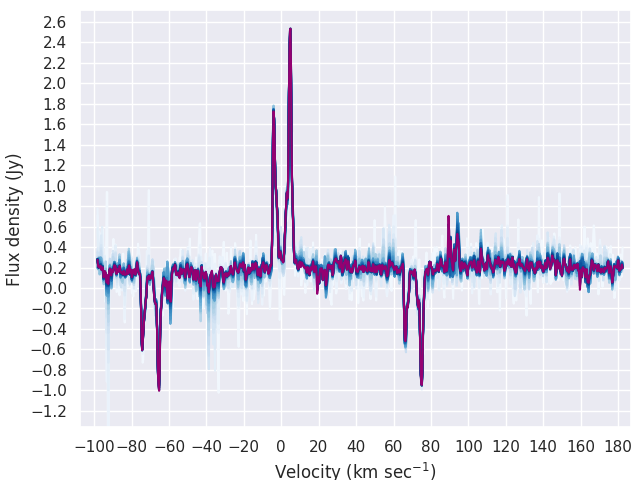
\includegraphics[width=\textwidth]{images/created/rlmi-doppler.png}
\caption{Plūsmas blīvuma atkarība no objekta ātruma maiņzvaigznes RLMi kreisās cirkulārās polarizācijas datiem.}
\label{fig:rlmi-doppler}
\end{figure}
Izmantojot \ref{doppler} nodaļā aprakstīto metodiku, spektra frekvenču josla tiek pārrēķināta uz objekta ātruma vērtībām. Pēc datu apstrādes, rezultējošajā spektrā, ir iegūti pīķi -4 km/s un 5 km/s vērtībās, kas arī pēc aprēķiniem ir novērotā OH māzera pārvietošanās ātruma vērtības ar augstu trokšņa pret signāla attiecību.


\section{Bakalaura darba izstrādes laikā novērotie kosmiskie objekti} \label{objects}


Bakalaura darba ietvaros tika novēroti vairāki radioastronomiski objekti, kurus var iedalīt kategorijās - maiņzvaigznes, komētas un zvaigžņu veidošanās apgabali.

Novērojot vājus objektus, lai nodrošinātu datu integritāti, nepieciešams kāds spēcīgāks avots, kuru vieglāk detektēt. Bakalaura darba novērojumu ietvaros tika izmantota maiņzvaigzne R Leonis Minoris (turpmāk RLMi). Balsoties uz rakstu no Nancay radioastronomijas observatorijas Francijā, \cite{nancay} tika salīdzinātas iegūtās vērtības ar Irbenē iegūtajām un tika iegūts līdzīgs rezultāts. Kopš tā brīža, RLMi tika novērots visās novērojumu sesijās, kur tiek novērota komēta Saules sistēmā.

Iegūstot rezultātus uz salīdzinoši spēcīgā avota RLMi, bija iespējams novērot arī komētas Saules sistēmā, kuras izstaro vāju OH māzera starojumu. Pirmā novērotā komēta, kura tika apskatīta Bakalaura darba ietvaros ir Panstarrs C/2017 T2 (turpmāk Panstarrs). Ņemot vērā, ka objekta orbīta nodrošina ilgstošu redzamību, komēta ir novērota visilgāko laiku. Lai gan komēta ir salīdzinoši vāja spilgtuma - vidēji ap 12 magnitūdām pēc NASA HORIZONS datiem novērojumu veikšanas laikā, ilgais novērošanas laiks dod iespēju efektīvāk pārbaudīt ar vairāku novērojumu apvienošanu saistītu metodiku.

Asteroid Terrestrial-impact Last Alert System jeb ATLAS 2019 gada 28. decembrī atklāja jaunu komētu - ATLAS C/2019 Y4 (turpmāk Atlas). Gada beigās atklātajai komētai tika aprēķinātas augstas spilgtuma vērtības, kas sniedza iespēju daudziem zinātniekiem to novērot. Komētu klasificē kā Kreutz sungrazer tipa komētu, kas nozīmē, ka komētas perifērijas ir ļoti tuvu Saulei. Lai gan tas pozitīvi ietekmē komētas spilgtumu, tas palielina iespējamību komētām sadalīties, kas arī notika ar Atlas komētu ap 2020. gada 1. aprīli \cite{atlas-frag}.   Komētas orbīta liecina, ka Atlas komēta ir bijusi daļa no Lielās komētas C/1844 Y1 \cite{atlas-article}, bet atdalījusies aptuveni piecu tūkstošu gadu atpakaļ. Komētai sadaloties, stipri palielinās komētas spilgtums, taču sadalīšanās brīdī komētai veidojas vairākas daļas, kur nereti katrai daļai ir savs kodols. Kodolā esošo OH molekulu daudzums vairs nav tik daudz, līdz ar to starojuma jauda samazinās, kas noved pie samazinātām komētas novērošanas iespējām.

Lai gan Atlas komētas sadalīšanās nozīmēja komētas novērošanas beigas, Saules sistēmā parādījās jauna spoža komēta - SWAN C/2020. Pirmo reizi atklāta, izmantojot Solar and Heliospheric Observatory jeb $SOHO$. Swan komēta tika atklāta, jo tā izvadīja kosmosā ļoti lielu daudzumu $H_2O$ \cite{swan-disc}. Komēta Bakalaura darba nodevuma laikā joprojām tiek novērota un darbs pie datu apstrādes turpinās.

\begin{table}[h!]
\centering
\caption{Bakalaura darba izstrādes laikā ilgstoši novērotās komētas}.
\begin{tabular}{|c|l|l|l|l|l|}
\hline
\textbf{Objekta nosaukums} & \textbf{Atlas C/2019 Y4} & \textbf{Panstarrs C/2017} & \textbf{Swan C/2020 F8}  \\ \hline
\textbf{Tuvākā distance līdz Zemei} & 0.781 AU & 1.5202 AU  &  0.557 AU  \\ \hline
\textbf{Tuvākā distance līdz Saulei} & 0.253 AU & 	1.615 AU &  0.432 AU  \\ \hline
\textbf{Spilgtums perihēlija punktā}           & Sadalījusies & 8.6  &  7.6   \\ \hline
\textbf{Objekta novērojuma ilgums}       & 133h 16m 47s & 149h 21m 54s &  110h 09m 57s \\ \hline
\textbf{Novērojumu sākuma datums}       & 2020-Mar-14 & 2020-Jan-26 &  2020-May-05 \\ \hline
\textbf{Pēdējais novērojumu datums}       & 2020-Apr-11 & 2020-May-04 &  2020-May-20 \\ \hline

%\multicolumn{1}{|l|}{}                   &  &  &  &  &  &  &  &  &  \\ \hline
\end{tabular}

\label{tab:main-objects}
\end{table}

% Objekta nosaukums & Tuvākā distance līdz Zemei & Maksimālais spilgtums & Objekta novērojuma ilgums\\

Neskaitot primārās komētas, kuras aprakstītas \ref{tab:main-objects} tabulā\footnote{Distances un spilgtuma dati no astro.vanbuitenen.nl}, tika arī novērotas sekojošās komētas: C/2018 N2 (ASASSN), C/2019 B1 (Africano), 284P/McNaught, taču minētie objekti bija pārāk vāji novērošanas laikā, vai bija tehniskas problēmas, kuras liedza veikt ilgstošus novērojumus.


%\begin{table}[h!]
%\centering
%\begin{tabular}{|c|l|l|l|l|l|}
%\hline
%\multicolumn{4}{|c|}{Mazāk novērotās komētas}                            \\ \hline
%\textbf{Objekta nosaukums} & \textbf{Mcnaught} & \textbf{Africano} & %\textbf{Assasn}  \\ \hline
%\textbf{Tuvākā distance līdz Zemei (KM)} &  &  &    \\ \hline
%\textbf{Tuvākā distance līdz Saulei (KM)} &  &  &    \\ \hline
%\textbf{Maksimālais spilgtums}           & ???  & ???  &  ???   \\ %\hline
%\textbf{Objekta novērojuma ilgums}       & ??? & ??? &  ??? \\ \hline
%\multicolumn{1}{|l|}{}                   &  &  &  &  &  &  &  &  &  \\ \hline
%\end{tabular}
%\caption{Bakalaura darbā novērotās komētas Saules sistēmā}
%\label{tab:min-objects}
%\end{table}


Bakalaura darba izstrādes laikā, tika novērotas ne tikai komētas Saules sistēmā, bet arī radioastronomiski māzeri, kas staro spēcīgāk par komētām. Viens no tiem bija metanola māzeris Cepheus A zvaigžņu veidošanās apgabalā. Balstoties uz to, ka objekts tika novērots jau iepriekš, bija zināms, ka tā pīķis sasniedz 180 Jy vērtību, līdz ar to, objekts tika izmantots, lai testētu jēldatu apstrādes algoritmu uz cita veida datiem. Spēcīgu māzeru novērojumos parasti nav nepieciešams izmantot jēldatu formātu, jo dat faili sniedz pietiekami labu precizitāti, līdz ar to metodika, kā apstrādāt māzeru jēldatus nebija izveidota, taču šajā datu līmenī, starpība starp objektiem ir ļoti maza, līdz ar to, var izmantot to pašu apstrādes procesu. Māzeru apstrāde sniedza iespēju efektīvāk identificēt kļūdas, jo spektram bija iepriekš zināma forma, ar ko varēja salīdzināt iegūtos datus, kas nav iespējams komētu novērojumiem.

Papildus minētajiem novērojumiem, Bakalaura darba izstrādes laikā tika novērots vēl viens vājš OH māzeris - g126p715 0p822, kurš tika izmantots līdzīgiem nolūkiem, bet rezultātiem būtu jābūt līdzīgākiem komētu OH māzeru novērojumu rezultātiem. Māzera novērošanas laiks bija ļoti īss, kā arī novērojumu laikā bija tehniskas problēmas, kuras neļāva iegūt vēlamos rezultātus. Izmantojot datus no minētā māzera, kā arī dienu iepriekš novērotās C/2019 B1 (Africano) komētas, varēja identificēt, ka teleskopā ir problēmas, jo bija izteikts troksnis konkrētās frekvenču vērtībās.




%Spēcīgs avots novērojumu testēšanai:

%\textbf{RLMi}

%Komētas:

%\textbf{PANSTARRS (C/2017 T2)}

%\textbf{ATLAS (C/2019 Y4)}

%Mazāk novērotās:

%\textbf{Mcnaught}

%\textbf{Africano}

%\textbf{Assasn}

%Galaktiskie māzeri:

%\textbf{cepa}

%\textbf{g126p715 0p822}

%Nākotne:

%\textbf{C/2020 F8 (SWAN), C/2020 F3 (NEOWISE), C/2019 U6, 2P/Encke}


%\textbf{aprakstīt visus objektus, kā arī kapēc tie tiek izmantoti}





